\section{Исследование методов организации процесса обработки данных в КХЭД} \label{experiment}

Конфиденциальное хранилище электронных документов, как и любая другая система, может быть представлено в виде совокупности модулей, выполняющих различные функции. %Так как документооборот -- детерминированный процесс, каждый этап которого может быть детально расписан, можно рассматривать такие этапы в отдельности. 
Для каждого модуля можно определить варианты реализации, исходя из особенностей его работы. Наибольший интерес будут представлять следующие модули:
\begin{itemize}
	\item модуль обеспечения совместной работы пользователей;
	\item модуль хранения истории внесённых изменений;
	\item модуль обнаружения ошибок при обработке документа;
	\item модуль авторизации.
\end{itemize}
Остальные модули (передачи данных, разграничения доступа,защиты хранилища от несанкционированного доступа) реализуются стандартными методами и не представляют такого интереса.

\vspace{\baselineskip}
Для выбора реализации модулей КХЭД в соответствии с показателями эффективностями, которые будут описаны позднее, необходимо провести экспериментальное исследование существующих реализаций подобных модулей. Так как СЭД дороги и сложны в развёртывании, не все компании предоставляют демо-версии своих продуктов. Но и в случае наличия демо-версии довольно сложно её получить и оценить параметры (часто вместо демо-версии предоставляется презентация, отсутствует доступ к отдельным модулям системы). Существует и ещё один фактор, затрудняющий сложность проведения эксперимента: так как СЭД является системой массового обслуживания, для её объективного тестирования необходимо провести множество однотипных испытаний, включающих в себя работу нескольких испытуемых (пользователей СЭД) в течение длительного времени.

\vspace{\baselineskip}
С учётом всех вышеизложенных ограничений, было принято решение првоести имитационное моделирвоание модулей КХЭД в среде AnyLogic, приняв за описание моделей базовые принципы построения исследуемых модулей в различных реализациях.

\subsection{Модуль обеспечения совместной работы пользователей} \label{research_competition}

При совместной конкурентной работе пользователей в системе электронного документооборота существует проблема синхронизации вносимых изменений. Так, два редактора, работая над одним документом (каждый со своим набором задач), во время внесения изменений блокируют работу друг друга, так как документ в рассматрвиаемом контексте --- ограниченный ресурс. В один момент времени возможно только одно внесение изменений, это показано на рис. \ref{img:graph_oldscheme}.
\begin{figure}[h!]
  \centering
  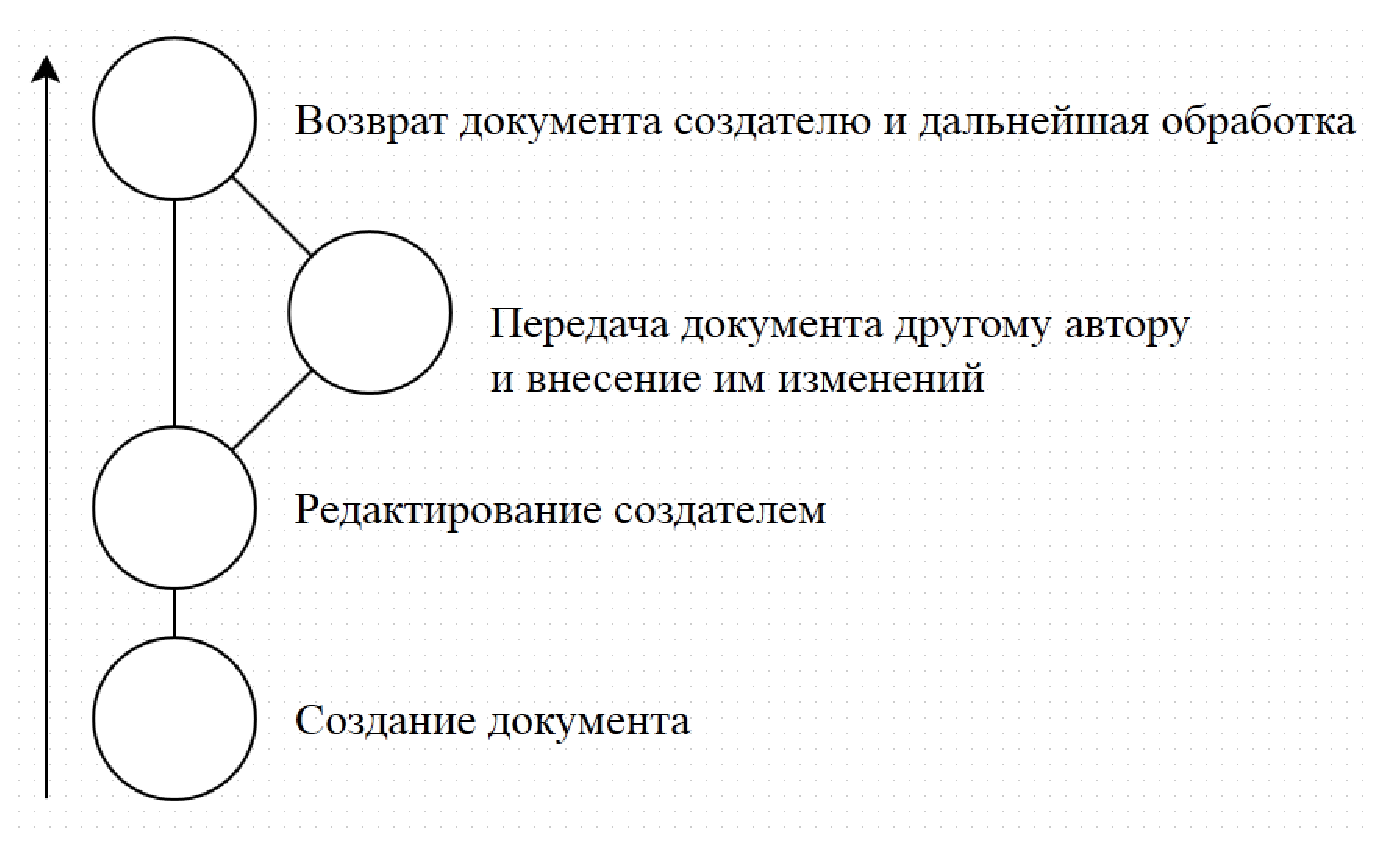
\includegraphics[width=0.7\textwidth]{graph_oldscheme}
  \caption{Схема конкурентной обработки документа с блокировкой}
  \label{img:graph_oldscheme}
\end{figure}

\vspace{\baselineskip}
Схема такой модели в среде AnyLogic представлена на рис. \ref{img:competition_old_scheme}.
\begin{figure}[h!]
  \centering
  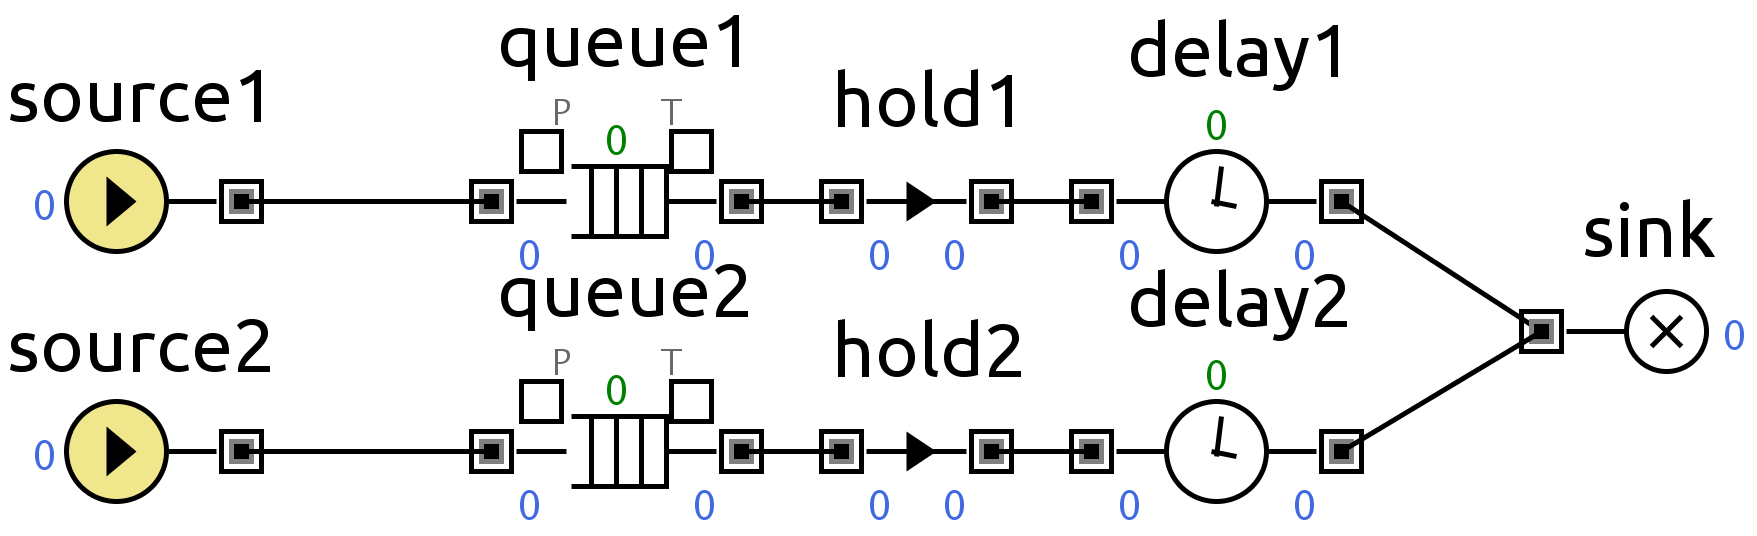
\includegraphics[width=0.7\textwidth]{competition_old_scheme}
  \caption{Модель обработки документа с блокировкой в среде AnyLogic}
  \label{img:competition_old_scheme}
\end{figure}

Здесь объекты $source$ моделируют источники заявок (по одной заявке в полчаса), $queue$ --- персональные очереди заявок на обработку, $hold$ --- элемент, блокирующий работу редактора (когда работает первый редактор, второй блокируется, и наоборот), $delay$ --- редакторы (время обработки заявки распределяется по нормальному закону со средним значением 25 минут, $\sigma=5$), $sink$ --- целевое хранилище, собирающее обработанные заявки.

\vspace{\baselineskip}
Альтернативой является такая схема организации обработки документов, при которой разрешено одновременное внесение изменений в документ, что справедливо для разрабатываемой системы --- см. рис. \ref{img:graph_newscheme}. Это становится возможным благодаря регистрации не состояний документа, а вносимых в него изменений в виде разницы текущего и предыдущего состояний. Пример такой разностной записи показан на рис. \ref{img:git_patch}.

\begin{figure}[h!]
  \centering
  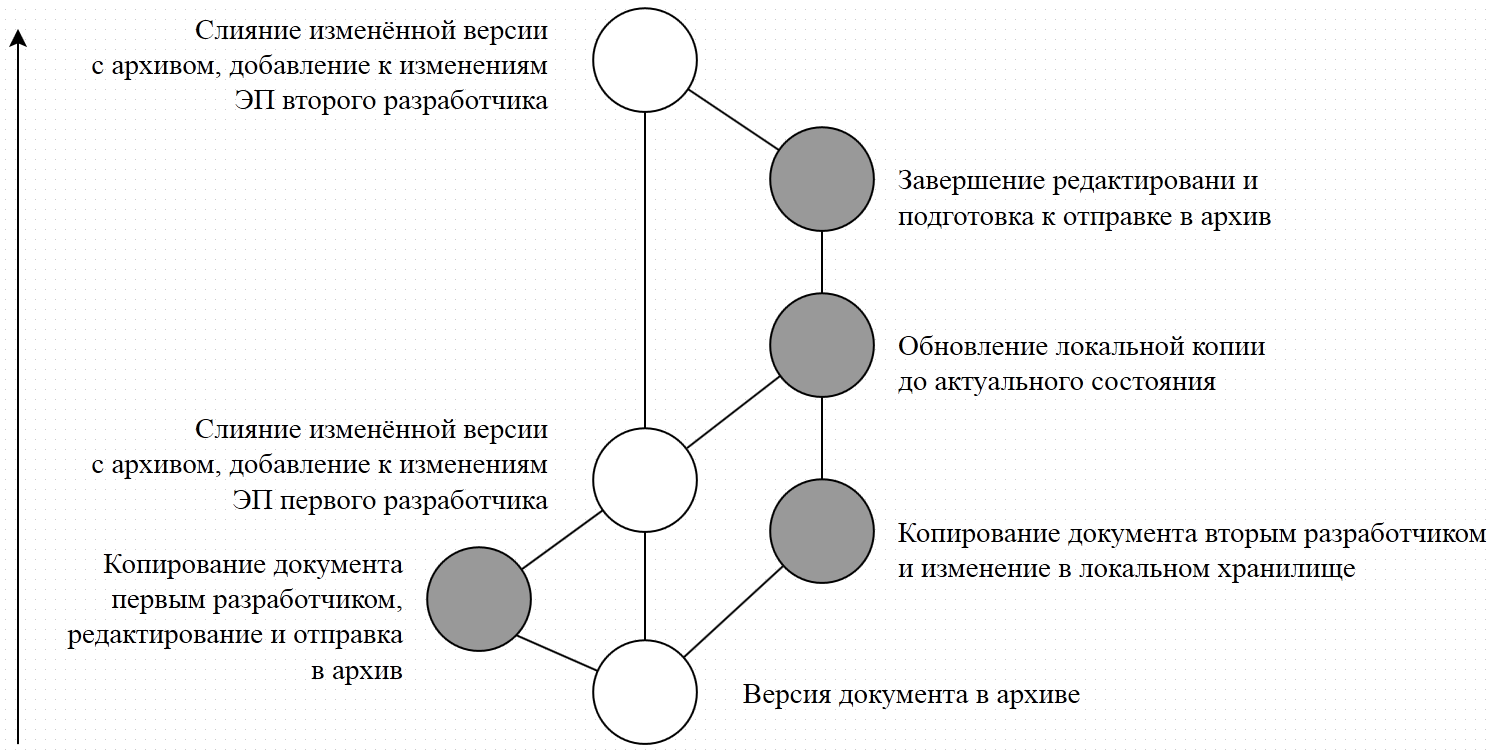
\includegraphics[width=1\textwidth]{graph_newscheme}
  \caption{Схема конкурентной обработки документа без блокировки}
  \label{img:graph_newscheme}
\end{figure}

\begin{figure}[h!]
  \centering
  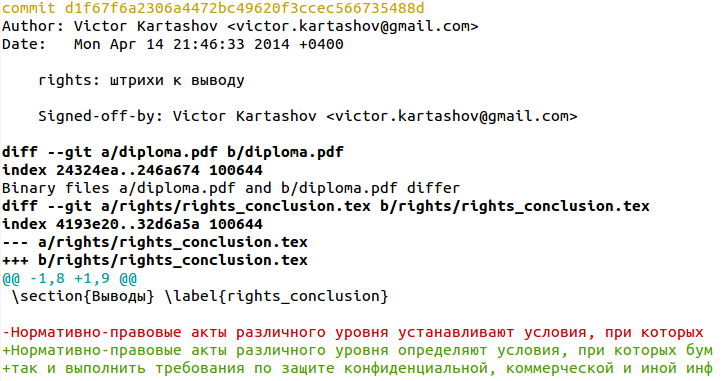
\includegraphics[width=0.8\textwidth]{git_patch}
  \caption{Пример описания состояния документа в виде разностной записи}
  \label{img:git_patch}
\end{figure}

Подобная структура может быть представлена в удобном для восприятия человеком виде, как показано на рис. \ref{img:git_meld}.
\begin{figure}[h!]
  \centering
  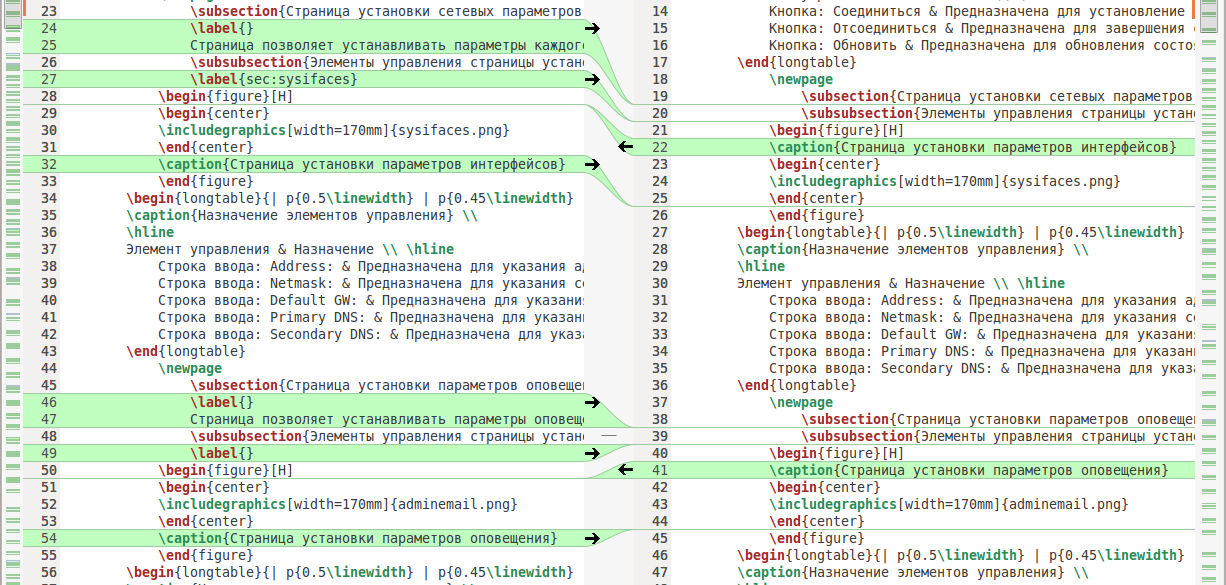
\includegraphics[width=1\textwidth]{git_meld}
  \caption{Пример представления разностной записи в виде постраничного сравнения}
  \label{img:git_meld}
\end{figure}

Данная реализация позволяет не только сократить объём хранимых данных, но и реализовать вышеописанную схему, ведь при таком подходе одновременное внесение изменений несколькими редакторами рассматривается не как изменение одного документа, а как создание набора новых записей. Результирующий документ получается путём последовательного применения таких <<патчей>> к исходному документу.

\vspace{\baselineskip}
Схема этой модели в среде AnyLogic представлена на рис. \ref{img:competition_new_scheme}.

\begin{figure}[h!]
  \centering
  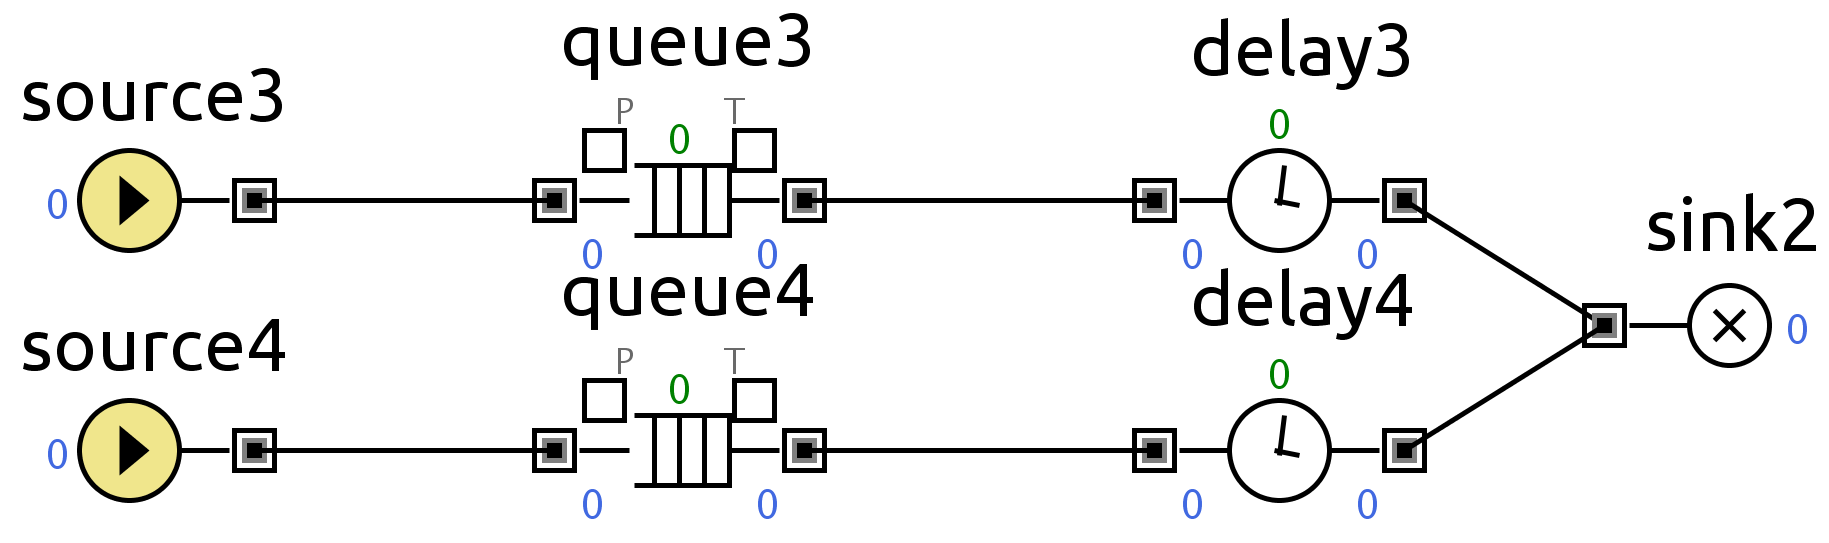
\includegraphics[width=0.7\textwidth]{competition_new_scheme}
  \caption{Модель обработки документа без блокировки в среде AnyLogic}
  \label{img:competition_new_scheme}
\end{figure}

\vspace{\baselineskip}
Элементы на этой схеме совпадают с элементами схемы рис. \ref{img:competition_old_scheme}, однако здесь отсутствуют блоки $hold$, а время обработки заявки распределяется по нормальному закону со средним значением 30 минут, $\sigma=6$ (из расчёта временного запаса на устранение ошибок слияния при одновременном переходе обработанных заявок в блок $sink$).

\vspace{\baselineskip}
В процессе эксперимента был промоделирован один рабочий день (с 9:00 до 18:00), в течение которого каждому из редакторов на обработку поступило 19 заявок. Число обработанных заявок в схеме с блокировкой показано на рис. \ref{img:competition_old_done}, в схеме без блокировок --- на рис. \ref{img:competition_new_done}.

\begin{figure}[h!]
  \centering
  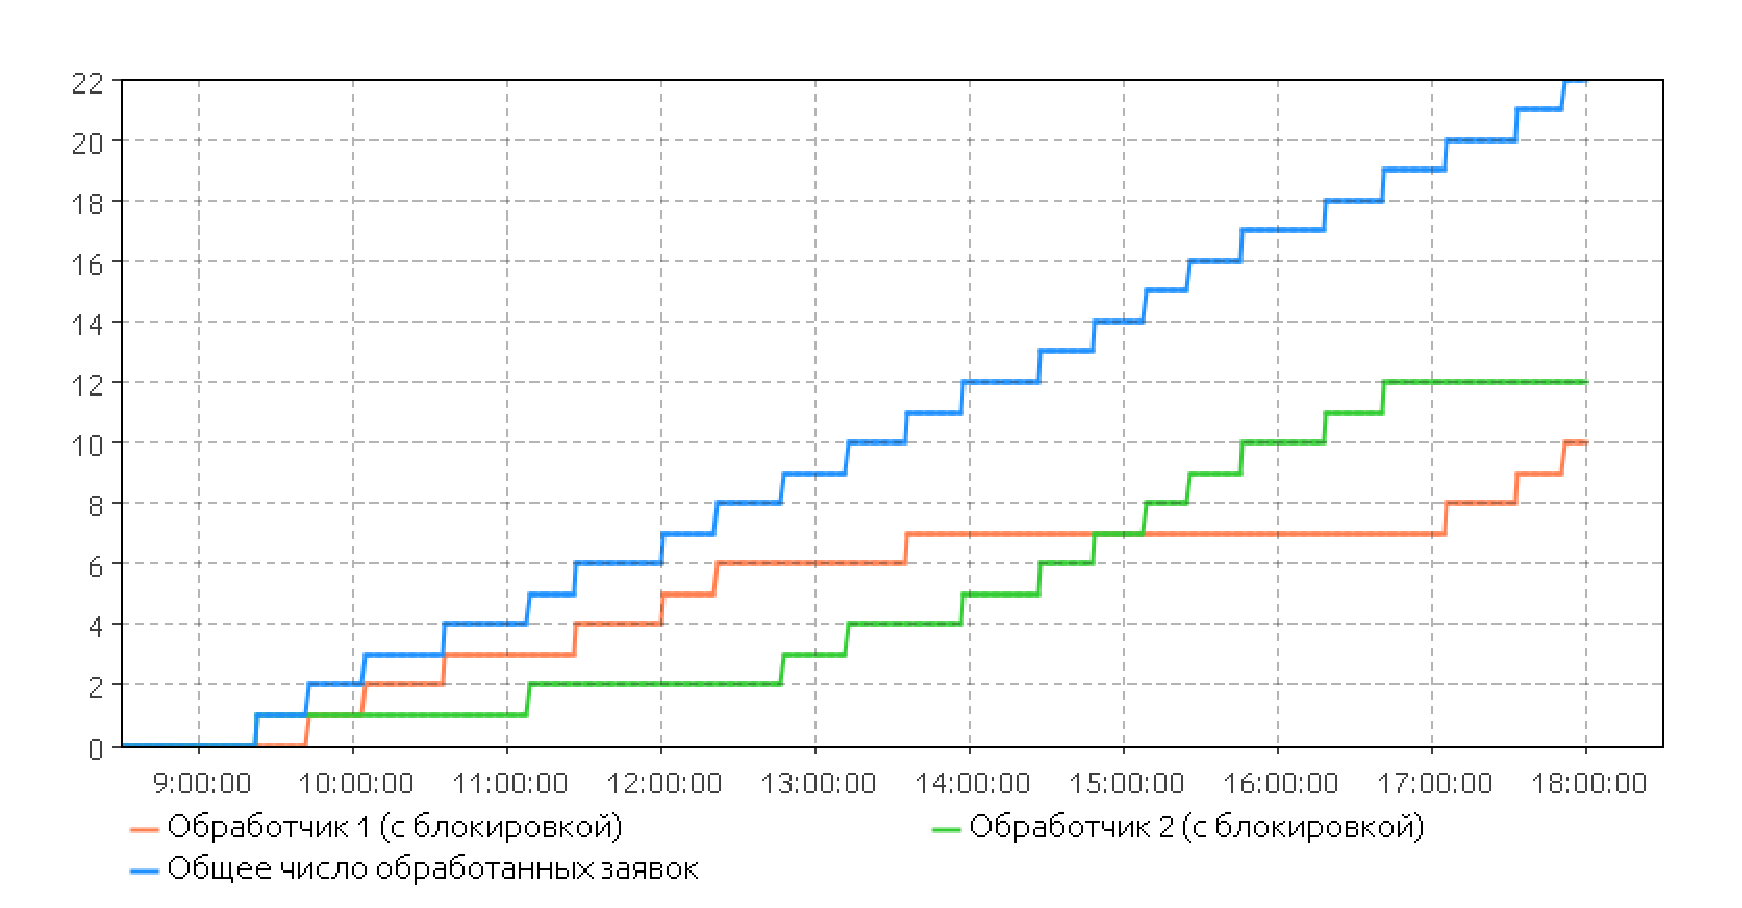
\includegraphics[width=1\textwidth]{competition_old_done}
  \caption{Число обработанных заявок в схеме с блокировкой}
  \label{img:competition_old_done}
\end{figure}

\begin{figure}[h!]
  \centering
  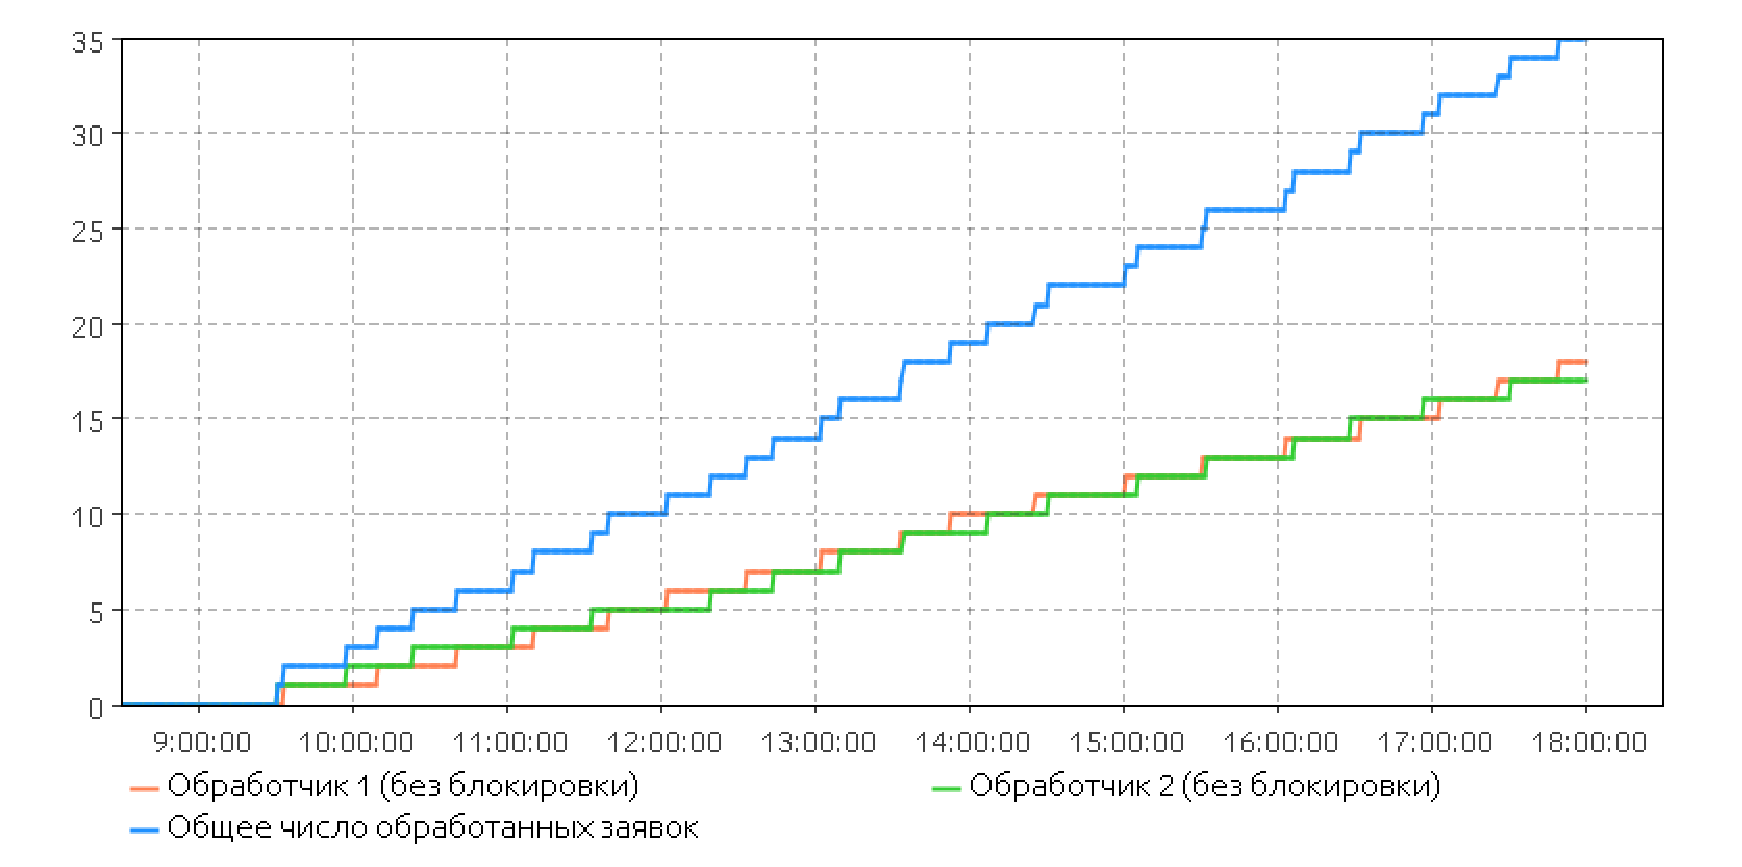
\includegraphics[width=1\textwidth]{competition_new_done}
  \caption{Число обработанных заявок в схеме без блокировки}
  \label{img:competition_new_done}
\end{figure}

\vspace{\baselineskip}
Как видно из представленных результатов, несмотря на б\'{о}льшее среднее время обработки одной заявки число успешно обработанных заявок в схеме без блокировки за один рабочий день в $~1.5$ раза больше, чем число успешно обработанных заявок в схеме с блокировкой за тот же период. Также по этим рисункам видно, что за счёт блокировок заявки в первой схеме обрабатывались неравномерно, в отличие от второй схемы. Дополнительным подтверждением этому служат временн\'{ы}е диаграммы загруженности редакторов в течение рабочего дня, представленные на рис. \ref{img:competition_old_gantt} и \ref{img:competition_new_gantt}.

\begin{figure}[h!]
  \centering
  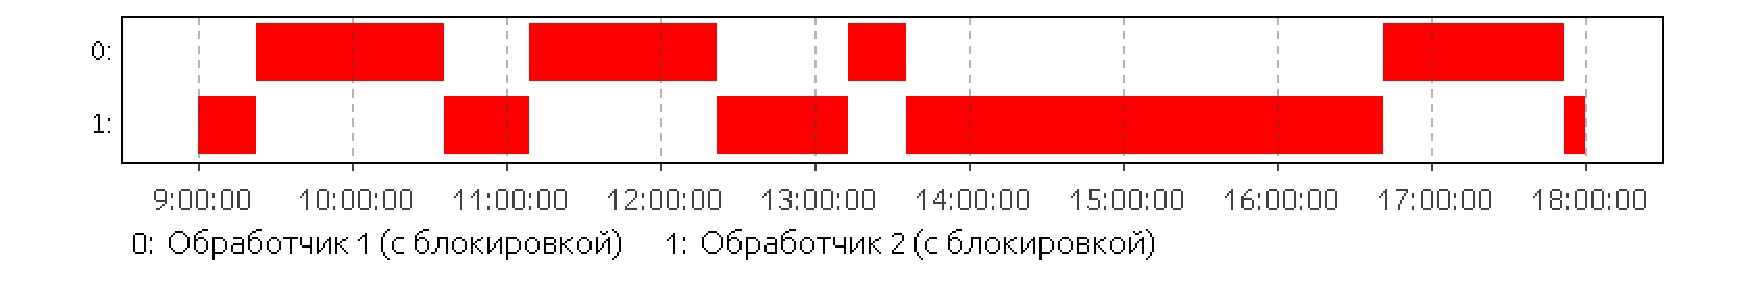
\includegraphics[width=1\textwidth]{competition_old_gantt}
  \caption{Временная диаграмма загруженности редакторов в течение рабочего дня в схеме с блокировкой}
  \label{img:competition_old_gantt}
\end{figure}

\begin{figure}[h!]
  \centering
  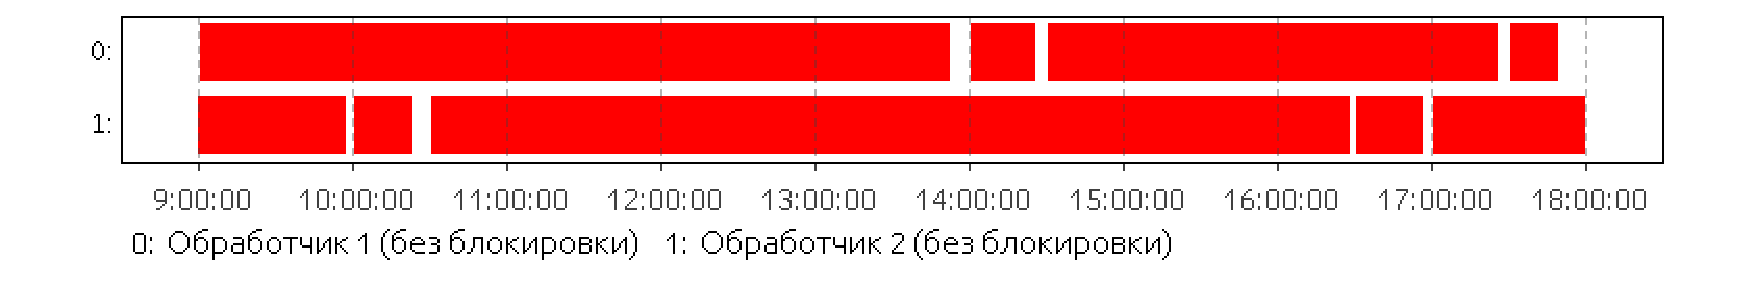
\includegraphics[width=1\textwidth]{competition_new_gantt}
  \caption{Временная диаграмма загруженности редакторов в течение рабочего дня в схеме без блокировки}
  \label{img:competition_new_gantt}
\end{figure}

\vspace{\baselineskip}
Данные рисунки наглядно показывают время бездействия редакторов в схеме с блокировкой (два редактора работают с загрузкой, равной 100\% загрузке одного редактора). Такого продолжительного простоя можно избежать только обрабатывая параллельно несколько документов разными редакторами так, чтобы время блокировок сводилось к минимуму. Таким образом, появляется дополнительная задача временн\'{о}го планирования. При этом схема без блокировок помогает эффективно использовать рабочее время без дополнительного планирования.

\vspace{\baselineskip}
Ещё один немаловажный показатель --- загруженность очереди на обработку. Соответствующие графики приведены на рис. \ref{img:competition_old_queue} и \ref{img:competition_new_queue}.

\begin{figure}[h!]
  \centering
  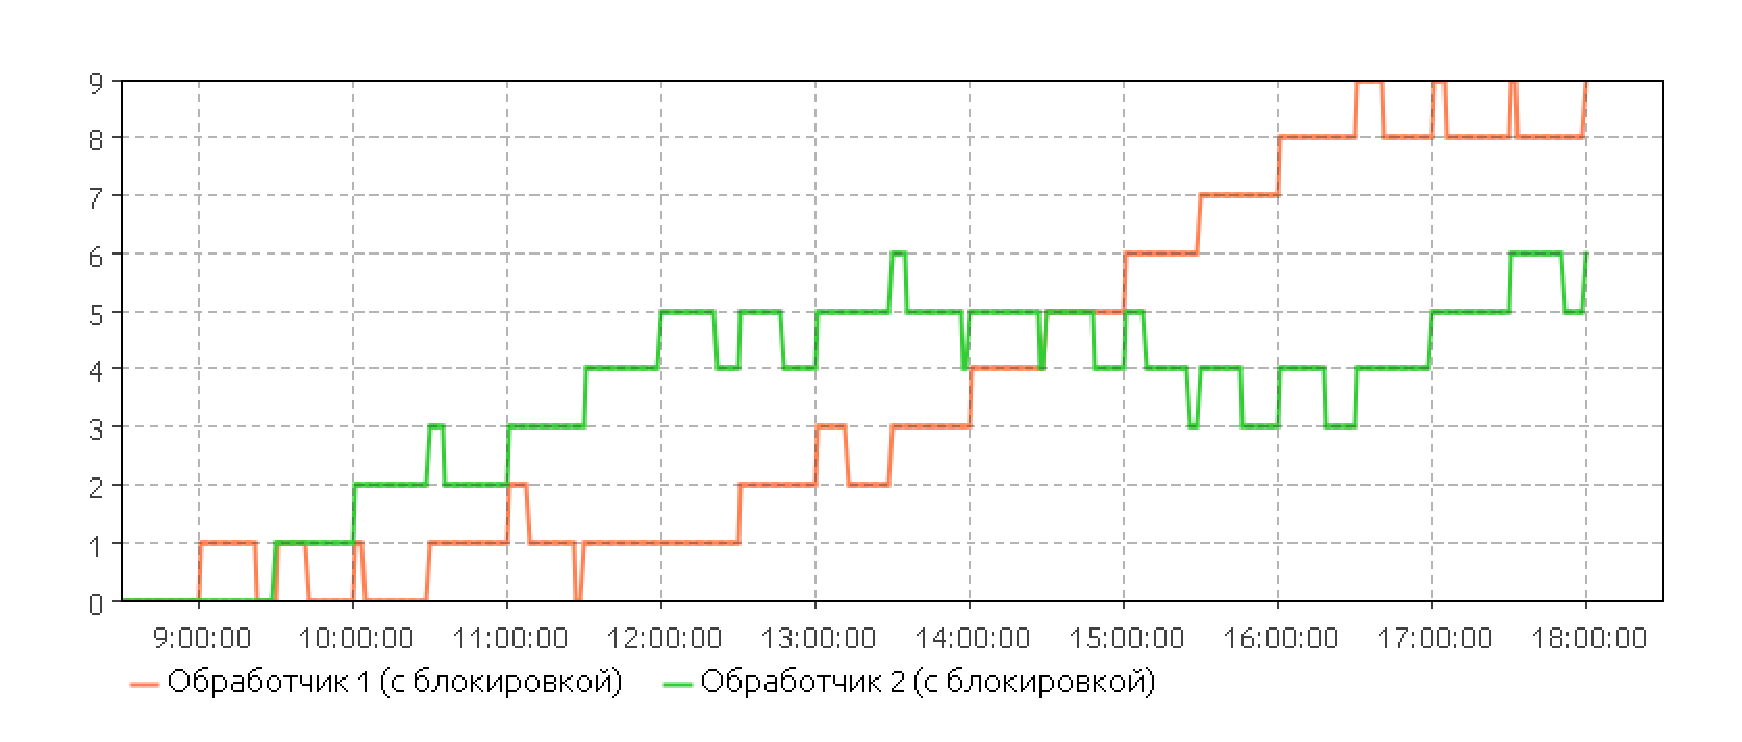
\includegraphics[width=1\textwidth]{competition_old_queue}
  \caption{Загруженность очереди на обработку в схеме с блокировкой}
  \label{img:competition_old_queue}
\end{figure}

\begin{figure}[h!]
  \centering
  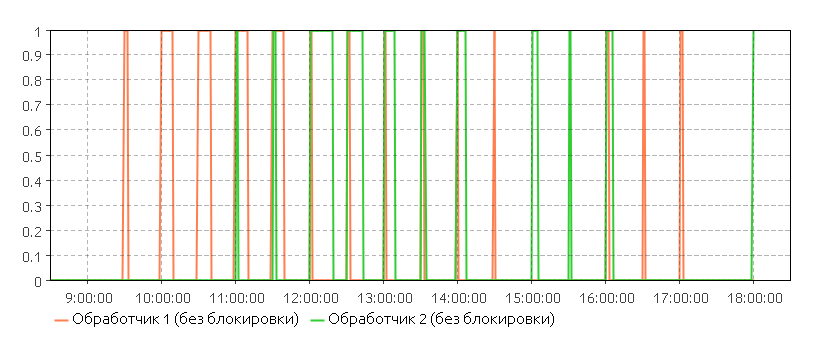
\includegraphics[width=1\textwidth]{competition_new_queue}
  \caption{Загруженность очереди на обработку в схеме без блокировки}
  \label{img:competition_new_queue}
\end{figure}

\vspace{\baselineskip}
Как видно, при использовании схемы с блокировкой заполняемость очереди имеет тенденцию к росту, что в конечном итоге приведёт к ситуации, в которой заявки одного конкретного редактора будут полностью удовлетворены только по завершении всех работ остальными редакторами. В то же время, очереди в схеме без блокировок не имеют подобной тенденции и заявки, находящиеся в них, своевременно удовлетворяются.

\vspace{\baselineskip}
Таким образом, при совместной работе пользователей над одним документом в системе электронного документооборота целесообразно использовать предложенную схему организации процесса без блокировок.				% Конкурентная обработка документа